\section{Initial Planning}
In Fall of 2008. Dr. Mike Heroux identified a need for
the Trilinos framework to include some sort of GUI package. Dr. Heroux wanted 
to give users of the framework the ability to easily generate GUIs for their
programs, while still providing a good experience for the end user. Based on
previous GUI work done for the Tramonto project, a few initial problems were
identified:

	\begin{itemize}
		\item How would the GUI be laid out?
		\item Different types of parameters require different methods of input.
			How would we decide how we would obtain input for a particular
			parameter?
		\item What framework would we use to build the GUI?
		\item How would the application developer specify parameters for the
			GUI to obtain?
		\item How would the application developer specify dependencies between
		parameters. This was a crucial problem/needed feature that was identified in
		development of the Tramonto GUI.
	\end{itemize}

After some deliberation, the following initial solutions were decided upon:

	\begin{itemize}
		\item The GUI would be laid out in a hierarchical fashion as shown in
		Figure \ref{paramlistFigure}. Parameters organized into lists and sublists. This
		would allow for a clear organization of the parameters as well as
		intrinsically demonstrate the relationships between them.
		\begin{figure}
			\centering
			\begin{picture}(50,150)(0,0)
				\put(10,0){\line(0,1){145}}
				\put(0,150){${Parameter List}$}
				\put(10,130){\line(1,0){15}}
				\put(28,127){$Parameter$}
				\put(10,110){\line(1,0){15}}
				\put(28,107){$Parameter$}
				\put(10,90){\line(1,0){15}}
				\put(28,87){$Parameter$}
				\put(10,70){\line(1,0){15}}
				\put(28,67){$Parameter List$}
				\put(38,0){\line(0,1){62}}
				\put(38,47){\line(1,0){15}}
				\put(56,44){$Parameter$}
				\put(38,22){\line(1,0){15}}
				\put(56,24){$Parameter$}
			\end{picture}
			\caption[GUI Layout]{The hierarchical layout of the GUI}
			\label{paramlistFigure}
		\end{figure}
		\item It be required that all parameters specify their type and the
		following types would be accepted:
			\begin{itemize}
				\item int
				\item short
				\item float
				\item double
				\item string
				\item boolean
				\item arrays of int, short, double, and string
			\end{itemize}
		For number types, a spin box would be used as input. If the valid
		values for a string type were specified, a combo box would be used.
		Otherwise a line edit would be used. For booleans, a combo box would
		also be used. For arrays, a pop-up box containing numerous input
		widgets would be used. The widget type would be determined by the
		array type.
		\begin{figure}[h]
			\centering
			\subfigure[A Spin Box]{
				\label{spinboxfig}
				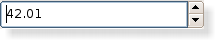
\includegraphics[scale=0.5]{graphics/spinbox}
			}
			\subfigure[A Combo Box]{
				\label{comboboxfig}
				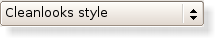
\includegraphics[scale=0.5]{graphics/combobox}
			}
			\subfigure[A Line Edit]{
				\label{lineeditfig}
				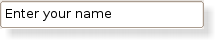
\includegraphics[scale=0.5]{graphics/lineedit}
			}
			\caption{Some of the various widgets used for editing data}
			\label{editingWidgets}
		\end{figure}

		\item QT was chosen as the GUI framework for several reasons:
			\begin{itemize}
				\item It is cross-platform.
				\item It is mature and has a well developed set of
				development tools.
				\item It has a rich feature-set.
				\item It has been used by Sandia in the past.
				\item The Optika developer was familiar with it.
			\end{itemize}
		\item Initially it was decided that the application developer would
		specify parameters via an XML file. A DTD would be created specifying
		the legal tags and name spaces.
		\item Dependencies would be handled through special tags in the DTD.
	\end{itemize}

\section{Early Development}
The first several months of development were spent on creating and implementing the XML
specification. The name of the XML specification went through several revisions but was
eventually called Dependent Parameter Markup Language (DPML).

After several months of development it was realized that creating an entirely new way of specifying 
parameters might hinder it's adoption. It pointed out that Trilinos actually had
a ParameterList~\cite{ParameterList} class in the Teuchos package. The ParameterList seemed to be better than DPML for
several reasons:
	\begin{itemize}
		\item It was already heavily adopted.
		\item It had the necessary hierarchical nature.
		\item It was serializable to and from XML.
	\end{itemize}

For these reasons, DPML was scrapped in favor of using Teucho's ParameterLists. Development moved
forward with the goal of creating a GUI framework that, in addition to meeting all the challenges 
outlined above, would also be compatible with any existing program using Teuchos's ParameterLists.

\section{Heavy development}
Starting in May 2009 a more heavy focus was put on development of the Trilinos GUI package.
With the back-end data-structure of the Teuchos's ParameterList already in place, attention
was turned to the developing the actually GUI itself. A key technology provided by Qt was it's Model/View
framework~\cite{QtModelView}. Using the Model/View paradigm, a wrapper class named TreeModel
~\cite{TreeModel} was created around the ParameterList class by subclassing the 
QAbstractItemModel~\cite{QAbstractItemModel}.

However, in subclassing the QAbstractItemModel it was realized that the ParameterList class fell short in
certain areas. At this point the main issue was that a given ParameterEntry~\cite{ParameterEntry} located within
a ParameterList or a given sublist located within a ParameterList was not aware of it's parent.
This was an issue because Qt's Model/View framework requires items within a model to be aware of
their parents. In order to circumvent this issue the TreeItem~\cite{TreeItem} class was created. Now 
instead of simply wrapping around a ParameterList class, the TreeModel created by giving it a ParameterList.
It would then read in the ParameterList and create a structure of TreeItems.  Each TreeItem then contained a pointer 
to it's corresponding ParameterEntry.

Once the TreeModel and TreeItem class were complete an appropriate delegate to go between and View
and the TreeModel was needed. A new class called Delegate~\cite{Delegate} was created to fill this
role by subclassing QItemDelegate~\cite{QItemDelegate}. As specified above, the delegate would return
the appropriate editing widget based on it's datatype.

With the model and delegate classes in place, an appropriate view could be applied. At first a simple
QTreeView~\cite{QTreeView} was applied to the model. The results was something like that in \ref{treeviewFig}.
	\begin{figure}[h]
		\centering
			\subfigure[A Tree View]{
				\label{treeviewFig}
				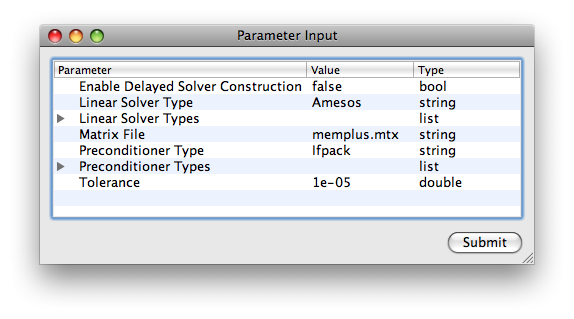
\includegraphics[scale=0.5]{graphics/treeview}
			}
	\end{figure}

Finally, the OptikaGUI class was created. It has one static function, getInput. A ParameterList is passed to this function, a
GUI is gereated, and all user input is stored in the ParameterList that was passed to the function. When the user hits the submit
button the GUI closes and the ParameterList that was passed to the getInput function now contains all of the user input.


\section{Advanced Features}
With the basic framework in place, we were now able to move on to more advanced features. As these advanced features
were developed various refactorings were made to the already existing code in order to support these new features.

	\subsection{Validators}
	One of the goals of Optika is to make life easier for the User. It's not enough to simply give the user information, it must
	be conveyed in a meaningful way. Validators are a great way of informing user what the valid set of values for a particular parameter are.
	Teuchos ParameterLists already came with built in validator functionality, but the default validators that were available
	were sorely lacking in capability. Three initial sets of validators were created to help deal with the short comings of
	the available validator classes:
	\begin{itemize}
		\item EnhancedNumberValidators allowed for validating various number types.
			\begin{itemize}
				\item Ability to set min and max.
				\item Ability to set the step with which the number value was incremented.
				\item Ability to set the precision with which the number value was displayed.
			\end{itemize}
		\item StringValidator allowed the specification of a particular parameter as only accepting string types 
		and allowed for specifying a valid list of values.
		\item ArrayValidators allowed for the all validator types to be applied to an array of values. The validator
		that is applied to each entry in the array is called the prototype validator.
	\end{itemize}
	A fourth Validator type, a FileNameValidator, was added later. This validator designates a particular string parameter
	as containing a file path and allows the developer to indicate that the file must already exist.

	By interrupting the these validators, Optika could either put certain restrictions on the input widget for a Parameter or change the
	type of input widget used entirely. For instance: with EnhancedNumberValidators the min, max, step, and precision of the
	EnhancedNumberValidator are all used to directly set their corresponding values in the QSpinBox class, but with the FileNameValidator
	a QFileDialog would appear instead of the normal QComboBox or QTextEdit used for string validators.

	\subsection{Dependencies}
	Many times the state of one parameter depends on the state of another. Common inter-parameter dependencies include:
	\begin{itemize}
		\item Visual Dependencies: One parameter may become meaningless when another parameter takes on a particular value.
		In this case the user no longer needs to be aware of the meaningless parameter and it's best to just remove it from
		their view so they don't potentially become confused. Visual dependencies allows the developer to express that "if this parameter 
		x takes on a particular value, then don't display parameter y to the user anymore."
		\item Validator Dependencies: Sometimes the valid set of values for one parameter changes if another parameter takes
		on a particular value. Validator Dependencies allows the developer to express that "if parameter x takes on this value, change
		the validator on parameter y."
		\item Validator Aspect Dependencies: Sometimes the developer doesn't want to change the validator on a particular parameter, but
		rather just a certain aspect of it. Validator Aspect Dependencies allows the developer to express that "if parameter x takes on this value,
		change this aspect of the validator on parameter y in such a fashion as relating to the new value of parameter x"
		\item Array Length Dependencies: Sometimes the length of an array in a parameter changes based on the value of another parameter.
		Array Length Dependencies allows the developer to express that "if parameter x changes its value, change the length of the array
		in parameter y in such a fashion as relating to the new value of parameter x."
	\end{itemize}

	Coming up with a way for the developer to easily express these concepts was not easy. Eventually, it was decided that a data structure called
	a dependency would hold all the dependencies used for a certain parameter list. Each dependency would at minimum specify the dependent parameter,
	the dependee parameter. However, a complication arose. Because we wanted dependencies to be able to have arbitrary dependents and dependees, we needed
	a way to uniquely identify the dependee and the dependent. While within a particular parameter list names of parameters are unique, names are not 
	necessarily unique across a set of sublists. Therefore, in order to uniquely identify a parameter and allow dependencies across sublists we would need
	to know both the parameter name and the parent list containing it\footnote{The astute reader will notice that if there are two sublists with different parent lists 
	and each sublist has a parameter with the same name, then we will not be able to uniquely identify the dependent and the dependee. This is such an edge case that we decided
	to ignore it and not implement any way to handle it}. So it became that every dependency, along with needing the names of the dependee
	and dependent, also needed their respective parent lists. The dependency sheet also needed the root list which contained all of the dependees and dependents.
	This was so we could recursively search for the parameters and their parent sublists (the only way to find them using our method of identification). 

	The Dependency classes were created to address the use cases above:
	\begin{itemize}
		\item Dependency
		\begin{itemize}
			\item NumberArrayLengthDepednency
			\item NumberValidatorAspectDependency<T>
			\item ValidatorDependency
			\begin{itemize}
				\item BoolValidatorDependency
				\item RangeValidatorDependency<T>
				\item StringValidatorDependency
			\end{itemize}	
			\item VisualDependency
			\begin{itemize}
				\item BoolVisualDepedency
				\item NumberVisualDependency<T>
				\item StringVisualDependency
			\end{itemize}
		\end{itemize}
	\end{itemize}

	Some of these Dependencies have some sick-awesome capabilities. Namely, the NumberArrayLengthDepednency, NumberValidatorAspectDependency, and NumberVisualDependencies
	can all take a pointer to a function as an argument. In the case of the NumberArrayLengthDepednency, this function can be applied to the value of the dependee
	parameter. The return value of this function is then used as the length of the array for the dependent parameter. For NumberValidatorAspectDependencies, the function
	is used to calculate the value of the chosen validator aspect. And in the NumberVisualDepenency class, if the function returns a value greater than 0 the dependent is
	displayed. Otherwise, the dependent is hidden. 

	The algorithm for expressing dependencies in the GUI is as follows:
	\begin{enumerate}
		\item A parameter's value is changed by the user.
		\item The Treemodel goes asks the dependency sheet associated with it if there parameter that changed has any dependents
		\item If the parameter does have dependents, the Treemodel requests a list of all the dependencies in which the changed
		parameter is a dependent
		\item For each dependency, the evaluate function is called. The dependency makes any necessary changes to the dependent parameter
		and the Treemodel updates the Treeview with the new data.
		\item If any dependents now have invalid values, focus is given to them and the user is requested to change their value to
		something more appropriate.
	\end{enumerate}

	\subsection{Custom Functions}
	Normally in Optika the user configures the parameter list, hits submit, the GUI disappears, and the program continues with execution. However,
	an alternative to this work flow was desired. A persistent GUI was needed. We added the ability to specify a pointer to a pointer to a function
	that would be executed whenever the user hit submit. The function needed to have the signature foo(Teuchos::RCP<const ParameterList> userParameters).

	\subsection{Various Niceties}
	Various niceties were added to the GUI as well. The ability to save and load parameter lists was added. The Optika GUI class was expanded to allow for
	customization of the window icon and use of Qt Style Sheets to style the GUI. Checks were also added so that if the user tried to exit the GUI without
	saving they would be warned and given the option to save their work.

\section{Waiting For Copyright}
	All of the above features were completed around the end of August 2009 and Optika was official given its name.
	Optika was submitted for copyright shortly after. I took Optika a little over six months to complete copyright.
	Since it was not copyrighted, it could not be included in the Trilinos 10 release. This made the primary developer extraordinarily
	angry and he tried very hard to contemplate what could possibly be taking so long. During the time Optika spend in copyright limbo, 
	little development on Optika was done. Most of development was cleaning up various paces of code, adding examples, and adding documentation. 
	Finally, in March 2010 Optika was ready to be included in Trilinos and was released to the public with the Trilinos 10.2 release.

\section{User Feedback}
In the summer of 2010, Optika got it's first user. Dr. Laurie Frink began using Optika to create a GUI for here program Tramonto.
Initial feedback was very positive. Laurie is a C programmer and while she had some issues picking up Optika (which is C++ based)
most were easily handled. Her questions also lead to the creation of some great examples. For the most part Dr. Frink found Optika
to be quite adequate for her purposed. However, Dr. Frink did have one rather major feature request: she needed the ability to 
specify multiple dependents and in some cases even multiple dependees. This was quite a task and required a large reworking of the
Dependency class. 

Adding support for multiple dependents wasn't that hard. Instead of specifying a single dependent to the constructor of a Dependency, a list
of Parameters was passed now. If the developer only needs one dependent then he/she can just pass a list of length one. A list simple
list worked in the case of all the dependents having the same parent list. If they had different parent lists, then a more complex 
data structure which mapped parent lists to parameters would be used. Convenience constructors were also made for simple cases where
there was just one dependent. The algorithm used for evaluating dependencies changed very little with these modifications. The only addition
needed was and extra loop for evaluating each dependent in a dependency for a given dependee.

Adding support for multiple dependents was much harder. There was actually only one specific use case that needed multiple dependents. Dr.
Frink needed the ability to test the condition of multiple parameters to determine whether or not a particular parameter should be displayed.
So a new VisualDependency class was created called ConditionVisualDependency. ConditionVisualDependencies evaluated a condition object to
determine the whether or not a set of dependents should hidden or shown. The set of condition classes created are as follows:
\begin{itemize}
	\item A ParameterCondition examines the value of a particular parameter and evaluates to true or false accordingly. Types of ParameterConditions include:
	\begin{itemize}
		\item BoolCondition examines boolean parameters.
		\item NumberCondition<T> examines number parameters.
		\item StringCondition examines string parameters.
	\end{itemize}
	\item A BinaryLogicalCondition examines the value of two or more conditions passed to it and evaluates to true or false accordingly. Types of BinaryLogicalConditions include:
	\begin{itemize}
		\item AndCondition returns the equivalent of performing a logical AND on all conditions passed to it.
		\item EqualsCondition returns the equivalent of performing a logical EQUALS on all conditions passed to it.
		\item OrCondition returns the equivalent of performing a logical OR on all conditions passed to it.
	\end{itemize}
	\item A NotCondition examines the value of one condition passed to it and evaluates to the opposite of what ever that condition evaluates.
\end{itemize}
Through the recursive use of BinaryLogicalConditions the developer can now chain together an arbitrary amount of dependents together.

ConditionVisualDependencies are the only dependencies which allow for multiple dependents. So while support was added for multiple depdents at the
Dependency parent class level, ConditionVisualDependency is the only class which actually implements the functionality. In this case the algorithm
for evaluating dependencies didn't need to change at all.

At the time of this publication, the Optika team is still waiting to hear back from Dr. Frink as to whether or not these new features met her needs.

\section{Future Development}
There are two main development goals for Optika in the near future. The first is to be able to completely write and Optika GUI (with dependencies and validators)
solely in XML. This requires that XML serialization for all of the validator and dependency related classes be developed. Currently,
XML serialization for validators is almost finished after which serialization for the dependency and dependency sheet class will begin.

The second goal is to develop stand-alone version of Optika. The development team believes that the potential audience for Optika is much 
larger than just user base of Trilinos. However, creating a stand-alone version presents the problem of keeping source code consistent between
the Optika that exists in Trilinos and the stand-alone version. No doubt python scripting will come in handy when solving this problem.


	



	

